\section{eo\-Prop\-Combined\-Mon\-Op$<$ EOT $>$ Class Template Reference}
\label{classeo_prop_combined_mon_op}\index{eoPropCombinedMonOp@{eoPropCombinedMonOp}}
{\bf eo\-Mon\-Op}{\rm (p.\,\pageref{classeo_mon_op})} is the monary operator: genetic operator that takes only one {\bf EO}{\rm (p.\,\pageref{class_e_o})}  


{\tt \#include $<$eo\-Proportional\-Combined\-Op.h$>$}

Inheritance diagram for eo\-Prop\-Combined\-Mon\-Op$<$ EOT $>$::\begin{figure}[H]
\begin{center}
\leavevmode
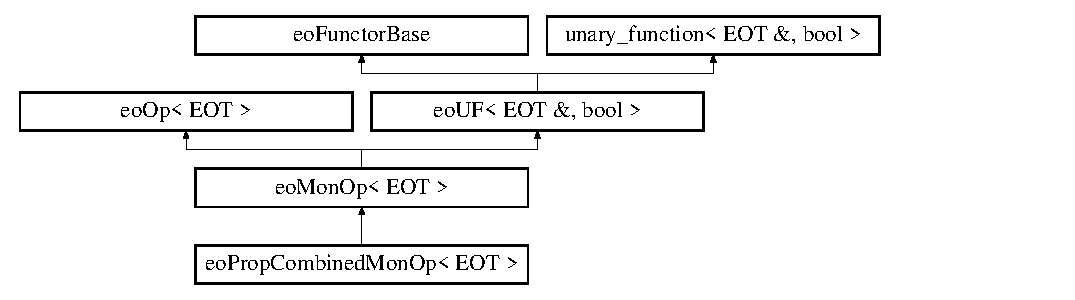
\includegraphics[height=3.58974cm]{classeo_prop_combined_mon_op}
\end{center}
\end{figure}
\subsection*{Public Member Functions}
\begin{CompactItemize}
\item 
{\bf eo\-Prop\-Combined\-Mon\-Op} ({\bf eo\-Mon\-Op}$<$ {\bf EOT} $>$ \&\_\-first, const double \_\-rate)\label{classeo_prop_combined_mon_op_a0}

\begin{CompactList}\small\item\em Ctor from a \char`\"{}true\char`\"{} operator. \item\end{CompactList}\item 
virtual std::string {\bf class\-Name} () const \label{classeo_prop_combined_mon_op_a1}

\item 
virtual void {\bf add} ({\bf eo\-Mon\-Op}$<$ {\bf EOT} $>$ \&\_\-op, const double \_\-rate, bool \_\-verbose=false)\label{classeo_prop_combined_mon_op_a2}

\item 
virtual void {\bf print\-On} (std::ostream \&\_\-os)\label{classeo_prop_combined_mon_op_a3}

\item 
virtual bool {\bf operator()} ({\bf EOT} \&\_\-indi)\label{classeo_prop_combined_mon_op_a4}

\begin{CompactList}\small\item\em The pure virtual function that needs to be implemented by the subclass. \item\end{CompactList}\end{CompactItemize}
\subsection*{Protected Attributes}
\begin{CompactItemize}
\item 
std::vector$<$ {\bf eo\-Mon\-Op}$<$ {\bf EOT} $>$ $\ast$ $>$ {\bf ops}\label{classeo_prop_combined_mon_op_p0}

\item 
std::vector$<$ double $>$ {\bf rates}\label{classeo_prop_combined_mon_op_p1}

\end{CompactItemize}


\subsection{Detailed Description}
\subsubsection*{template$<$class EOT$>$ class eo\-Prop\-Combined\-Mon\-Op$<$ EOT $>$}

{\bf eo\-Mon\-Op}{\rm (p.\,\pageref{classeo_mon_op})} is the monary operator: genetic operator that takes only one {\bf EO}{\rm (p.\,\pageref{class_e_o})} 

now accepts generic operators 



Definition at line 58 of file eo\-Proportional\-Combined\-Op.h.

The documentation for this class was generated from the following file:\begin{CompactItemize}
\item 
eo\-Proportional\-Combined\-Op.h\end{CompactItemize}
